\chapter{Approach}\label{chap:approach}
The approach starts with the problem definition and continues with the presentation of the ACO algorithm Ant-Power-Medium-Voltage for solving it.

\section{Optimization Problem}\label{optiproblem}
The goal of the ACO algorithm in grid planning is to connect the loads and generators of the grid in the most cost effective way whilst satisfying the side constraints. The topological side constraint is the n-1 criterion which requires every bus to be reachable via at least one alternative route. This resembles a ring structure in the graph (multiple rings are also valid). As described in \ref{ant_graph}, this can be done via finding the spanning tree of the ant graph which results in the lowest cost of its hull. The process of building the spanning tree can already stopped, if all stations of the network are covered. There already exist several algorithms to find a minimum spanning tree like Boruvkas algorithm in polynomial time ($O(mlogn)$, where $m$ is the number of edges and $n$ the number of vertices.) Unfortunately, this problem differs from the simple minimum spanning tree problem because not the cost of the ant edges but the cost of the hull of the spanning tree has to be minimized. Trying to deduce the cost of the ant edges from the cost of the hull is impossible since the edge weight depends on the node from which the edge is expanded. This can be illustrated in Figure \ref{fig:different_cost}.
\begin{figure}[h]
	\begin{centering}
		{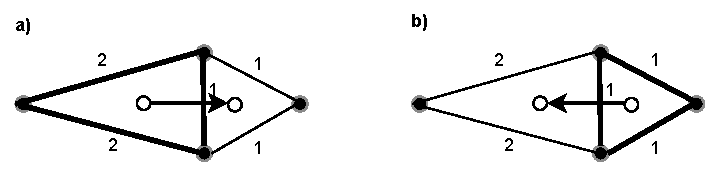
\includegraphics[scale=0.9]{figures/approach/different_cost.pdf}}
		\caption[Cost of ant edge]{The cost of an ant edge depends on the node from which it is getting expanded from.}
		\label{fig:different_cost}
	\end{centering}
\end{figure}
 \\
The left triangle has a cost of five, the right triangle a cost of three and their hulls when combined a cost of six. If the edge starts at the incenter of the left triangle and expands the right triangle additional cost of one are added to the hull ($5+3-2$, since the shared side of the triangles needs to be subtracted). Therefore, one could assign cost of one to the edge. But in the reverse case, the left triangle adds three to the cost of the hull ($3+5-2$).

Additionally, two electric side constraints need to be fulfilled. The maximum capacity of the power flow on a transmission line must never be exceeded. Similarly, the voltage violation limits of load buses in the network must be satisfied. In the case of MV grids in Germany according to DIN EN 50160 the voltage deviation at any bus at any time must not exceed a limit of  $\pm$ 5\%. The power that flows through a line segment shall never be more than 50\% of the lines capacity. To calculate the voltages and power flows in the network a power flow analysis is required.

%According to DIN EN 50160, under normal operating conditions, 95\% of the 10-minute average of the measured RMS value of each weekly interval must be within the limits of ±10\% of the nominal voltage.

%As inputs, PFA requires the impedances of lines and transformers, the voltages at sources, and the powers at sources, loads, and transformers
%TODO: check for exact electrical side constraint!

\section{Ant Power Medium Voltage}\label{sec:antpowermv}
The algorithm Ant Power Medium Voltage (APMV) was developed to solve the optimization problem formulated in the previous section. It is an advancement of the algorithm presented by Zeller in \cite{zeller2021planung} and uses concepts presented by Dorigo et. al. and Rotering.


%TODO: switch is in the middle of the ring
\subsection{Input and Parameters}\label{parameters}
The algorithm was specifically designed for the medium voltage level. If the input is a mixed grid and consists of multiple voltage levels, the medium voltage part needs to be extracted first (see \ref{sec:extraction}). As a data format the algorithm accepts a \textit{PyPSA}-network (see \ref{pypsa}) as an input file.\\
Important Parameters to set are the following:
\begin{itemize}
	\setlength\itemsep{-0.8em}
	\item \textbf{lineType}: Specifies the type of the line which should be build. This determines the lines resistance, reactance and capacity of its maximal power flow.
	\item \textbf{antsPerColony}: How many ants are building a solution in every iteration.
	\item {\boldmath{$q0$}: Probability that the ant chooses the best option (according to pheromone level + heuristic).
	\item \textbf{$\alpha$}: Parameter to determine the weight of the pheromones in the expansion decision.
	\item \textbf{$\beta$}: Parameter to determine the weight of the heuristic in the expansion decision.
	\item \textbf{$\rho$}: Parameter for the global pheromone update. Determines how much pheromone is deposited to reward the best solution.
	\item \textbf{$\xi$}: For the local pheromone update. Determines how much pheromone is removed from already used paths to evoke more exploration.}
	\item \textbf{iterations}: Number of iterations of the algorithm.
	\item \textbf{maximalRingsize}: Maximal number of buses allowed per ring.
\end{itemize}


\subsection{APMV Implementation}
In algorithm \ref{alg:high_level} the high-level implementation of the APMV is shown. At the very beginning, the input grid is prepared to work with the algorithm in a preprocessing step. Afterwards the initial pheromone is deposited. As already explained in Chapter \ref{chap:background}, every ant in the algorithm builds one solution per iteration. Out of these solutions the best one is kept and rewarded with pheromones which influences the solution building process of the next iteration ($globalPheromoneUpdate()$). At the end, the overall best solution and its cost is returned. $\varphi_0$ is the pheromone distribution at the start and $N$ is the number of stations in the network.

\begin{algorithm}[h]
	\caption{High-level implementation of APMV}
	\label{alg:high_level}
	\begin{algorithmic}[1]
		% \ttfamily
		\State $preprocessing$(grid) \alignedComment{extraction of mv grid and triangulation}
		\State $\varphi_0 \gets initializePheromones()$ \alignedComment{$\frac{1}{N}$, with $N$ number of stations}
		\State lowestCostSoFar $\gets \infty$ 
		\ForEach{i $\in$ iterations}
		\State $solutionsPerIteration \gets \emptyset$
		\ForEach{ant $\in$ antsPerColony}
		\State solution $\gets createSolution(\varphi_i)$
		\State solutionsPerIteration $\gets$ solutionsPerIteration $\cup$ solution
		\EndFor
		\State bestSolutionIter $\gets argmin$($cost$(), solutionsPerIteration)
		\If{$cost$(bestSolutionIter) < lowestCostSoFar}
		\State lowestCostSoFar $\gets cost$(bestSolutionIter)
		\State bestSolution $\gets$ bestSolutionIter
		\EndIf
		\State $\varphi_i \gets globalPheromoneUpdate$($\varphi_{i-1}$, bestSolution)
		\EndFor
		\State \Return bestSolution, lowestCostSoFar
	\end{algorithmic}
\end{algorithm}

\subsubsection{Global Pheromone Update}
%TODO: write formula
The global pheromone update is performed once after each iteration and deposits additional pheromones on the nodes expanded by the best solution found so far. Over time this enables the algorithms to learn from previous iterations which nodes generally lead to good or bad solutions. The formula for the global pheromone update on all visited nodes $i$ of the best solution is the following:
$$\varphi_i = (1-\rho) \varphi_i + \rho \frac{c_{est}}{c_{best}},$$
where $\rho \in (0,1)$, $c_{best}$ are the cost of the best solution found so far and $c_{est}$ are the estimated cost of the solution. The reciprocal of the $c_{best}$ is normalized by the $c_{est}$ to better reflect the quality of the solution. Low cost solutions receive high amounts of pheromone and vice versa.
%amount = estimated_min_expansion_cost / min_cost
%pheromone_i = pheromone_i * (1-rho) + amount * rho

\subsection{Solution Creation of Ants}
In algorithm \ref{alg:solution} the schematic implementation of the $createSolution()$ function is shown. The expanded nodes are ant nodes and the $solution()$ method checks whether the hull of the set expandedNodes covers all stations. The $expand()$ method finds the next node which should be added and depends on the pheromones $\varphi$, the heuristic $\eta$ and the neighborhood $neighbor()$ of the already expanded nodes. In the $localPheromoneUpdate()$, the pheromone gets decreased on the already used path to increase exploration and reduce the chance of convergence towards a local minimum. When $solution$(expandedNodes) is true, a solution is found and is returned with the updated pheromone level $\varphi$.
\begin{algorithm}[h]
	\caption{createSolution}
	\label{alg:solution}
	\begin{algorithmic}[1]
		% \ttfamily
		\State expandedNodes $\gets \emptyset$
		\While{$solution$(expandedNodes) $=$ false}
		\State newNode $\gets$ $expand(\varphi, \eta, neighbor$(expandedNodes)
		\State expandedNodes $\gets$ expandedNodes $\cup$ $expand(\varphi, \eta, neighbor$(expandedNodes))
		\State $\varphi \gets$ $localPheromoneUpdate$(newNode, $\varphi$)
		\EndWhile
		\State \Return expandedNodes, $\varphi$
	\end{algorithmic}
\end{algorithm}

\subsubsection{Local Pheromone Update}
%TODO: write formula!
%self._triangulation.get_shallow_copy_graph().edges[edge]['pheromone'] = \
%self._triangulation.get_shallow_copy_graph().edges[edge]['pheromone'] * (1 - self._xi) + \
%self._xi * self._initial_pheromone
\subsubsection{Heuristic}
The purpose of the heuristic is to provide additional guidance for the ant when making the decision which node to expand next. Especially in earlier iterations when the algorithm has not learned much yet (via pheromones) the heuristic can lead to better quality solutions. The overall cost of a built solution is roughly proportional to the length of the rings. The aim is to estimate the additional cost of expanding a node, so the ant can chose the one with the lowest cost. When adding a node (which represents a triangle) the length of the ring increases by the perimeter of the triangle minus two times the shared side (see Figure \ref{fig:heuristic} a)).
\begin{figure}[h]
	\begin{centering}
		{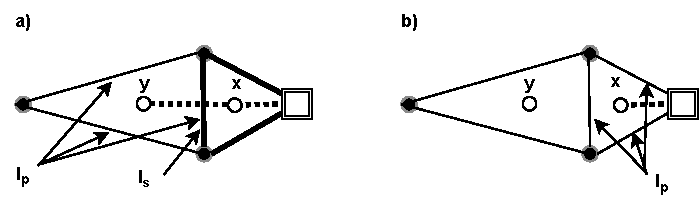
\includegraphics[scale=0.9]{figures/approach/heuristic.pdf}}
		\caption{Calculating the heuristic value.}
		\label{fig:heuristic}
	\end{centering}
\end{figure}
 \\
The reciprocal of the length a triangle (ant node) adds to the ring is used as a heuristic.
$$\eta_{x,y} = \frac{1}{l_{p} - 2l_{s}}$$
As explained in \ref{optiproblem} this heuristic not only depends on the expanded node $y$, but also on the node from which it gets expanded $x$. This leads to high heuristic values for triangles with short sides and low heuristic values for triangles with long sides. For the first triangle that gets expanded from the transformer node, the heuristic value is just the sum of the length of all sides, since there is no shared side (see Figure \ref{fig:heuristic}) b). The problem with this heuristic is that it does only minimizes the next expansion step and not the length of the ring at the end (greedy). Additionally, it does not account for the cost of voltage violations on buses.

\subsubsection{Expansion rule}
As shown in algorithm \ref{alg:solution}, the $expand()$ method depends on the heuristic $\eta$, the pheromones $\varphi$ and is limited to the neighbors of the already expanded ant nodes. As suggested by ACS \cite{ant_coloy_system}, the next node $s \in neighbor(x)$, with $x$ being the already expanded nodes and $s_i \in neighbor(x)$, is chosen according to the following rule:
$$p_s = \begin{cases}
	argmax_{s_i}(\varphi_{s_i}^\alpha \eta_{s_i}^\beta) & \, \text{, if q $\leq$} q_0\\
	\frac{\varphi_s^\alpha\eta_s^\beta}{\sum_{s_i}\varphi_{s_i}^\alpha\eta_{s_i}^\beta} & \, \text{, if q >} q_0
\end{cases}$$

where $q \in [0,1]$ is a uniformly distributed random variable. If the value of $q$ is greater than the threshold $q_0$ the algorithm choses the best known path (exploitation) and if $q$ is lower than $q_0$ the algorithm choses randomly (exploration). 

\subsection{Cost function}
The cost function plays a crucial part in the algorithm since it determines the pheromone distribution of the next iteration and therefore how the algorithm improves. The costs consist of two parts, the cost of building lines $b(x)$ and a penalty term for violations of electrical constraints $e(x)$.
$$cost(x) = b(d(x), c(x)) + e(x),$$
where $x$ is the network of the solution, $d(x)$ are the digging cost and $c(x)$ are the cable cost. The building cost and the penalty term will be discussed in more detail below.

\subsubsection{Building cost}
Concerning the cost of building lines, there are the acquisition costs of new transmission lines and the digging costs of laying the new cables into the ground. As an estimation for standard MV lines are taken cable cost of 130.000 Euro/km and digging cost of 100.000 Euro/km. These values of course fluctuate over time and have to be adapted for the specific situation. If the algorithm suggests building a line between two buses where a line already exists the costs are set to zero, assuming they can still be used in the future. For new transmission lines, the algorithms tries to predict the length and where the cable is laid along via the street network. Usually, cables are laid next to streets for better access and less invasive construction works. This is taken into account by using a tool developed by John, which uses data from open street map to find the distance and the path between two network stations along streets \cite{robert_john}. John first creates a graph from open street map in a given area, connects the network stations to it and then calculates the shortest path between the stations using Dijkstra. If the distance between two stations cant be estimated via open street map, the straight distance calculated via the haversine formula times $1.2$ is used.

\subsubsection{Penalty term}
The second part of the costs is a penalty term accounting for voltage violations of buses and loading violations of lines of the target grid. Therefore, a load flow analysis is conducted, which calculates the voltages and angles on all components of the network. If values exceed their limits penalties are added to the cost. These penalty costs are much greater in comparison to building costs. Thereby, the ants get rewarded much more by finding solutions without load flow violations. This almost guarantees that a convergence towards a solution has either no load flow violations at all or it is impossible to find a solution without it.

%TODO: check load flow analysis again!
%voltage deviations for buses
%loading violations for lines

\subsection{The Back-and-Forth Case}\label{backandforth}
As Zeller already points out in \cite{zeller2021planung}, there exist cases in which the standard process of building the hull  of the ant graph as described by Rotering does not work. Such a case is shown in Figure \ref{fig:backandforth}.
\begin{figure}[h]
	\begin{centering}
		{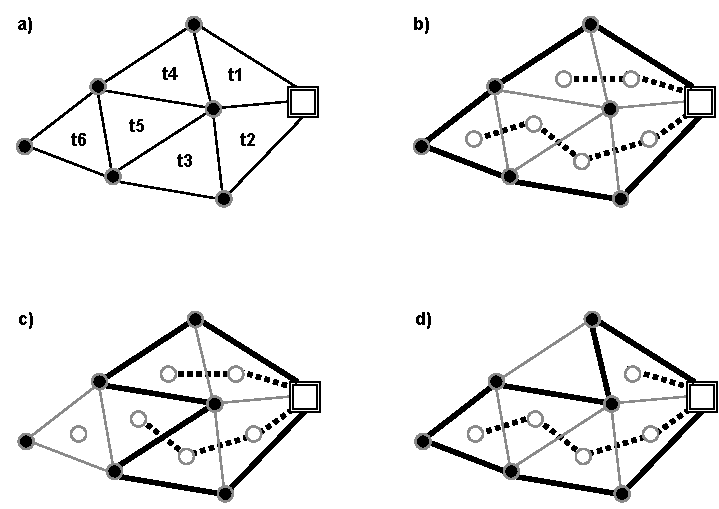
\includegraphics[scale=0.9]{figures/approach/backandforth.pdf}}
		\caption[Problematic case of building a ring]{Problematic case of building a ring via the hull of the ant graph.}
		\label{fig:backandforth}
	\end{centering}
\end{figure}

If the expansion of ant nodes proceeds as shown in case b) one station is not contained in the hull. The problem here is that it is possible to expand a triangle where all three stations are already covered by the hull at that point in time (t5 in c)). This is necessary though because the triangle t6 is only reachable via t5. Zeller's approach is to allow the expansion of the crucial triangle t5 anyways, but to do the routing in a way so it keeps the ring structure and it does not lose the connection to the node in the middle (Zeller called this a "back-and-forth" case). Unfortunately, his solution only worked in this specific case and did not cover further problems caused by the same issue. "Back-and-forth" cases can be chained indefinitely and Zeller only solved them until a certain depth. Another possible attempt of solving this issue would be to create two parallel lines from the hull to the unconnected station in the middle. This would maintain the ring structure but also connect the outer station twice. Therefore, APMV prohibits the expansion to triangles where all their three stations are already covered. If such a case occurs, the ant is getting restarted and a different solution is constructed (d). Depending on how often the ant needs to get restarted the performance of the algorithm decreases. During the creation of this work it was not clear how often such cases would appear in real networks and if it would be worth to develop an exact mechanism, which covers all problematic cases. For the real network example evaluated in this work however, a run of 1000 iterations and 15 ants per iteration only required 40 ants to be restarted, which does not represent a major issue ($\frac{40}{15000} = 0.00226 \%$). I leave for future work to find a method for an exact solutions to this problem.

\subsection{Multiple Rings}
For safety reasons it is common to limit the amounts of stations per ring to a certain number. Therefore, it is possible that multiple rings exist in the network. Another reason might be that rings connecting to different HV/MV transformers overlap in certain parts. Although it is possible to have multiple lines on the same path, the buses must only be connected to exactly one ring. To avoid the connection of buses to multiple rings it would be possible to check during the solution creation whether a bus is already covered by a different ring and to forbid its expansion. This however could lead to many dead ends, since the algorithm is limited to the expansion to neighboring nodes created by the triangulation. Therefore, APMV allows the rings to expand to every neighbor independent of their potential connection to a different ring and to resolve the issue in a post processing step.
\begin{figure}[h]
	\begin{centering}
		{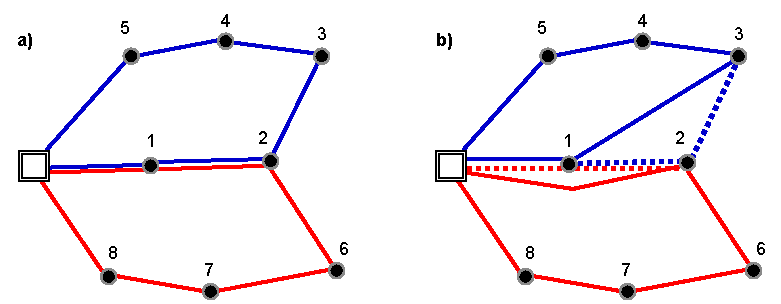
\includegraphics[scale=1]{figures/approach/busnosplit.pdf}}
		\caption{Handling of overlapping rings.}
		\label{fig:busnosplit}
	\end{centering}
\end{figure}

Figure \ref{fig:busnosplit} a) shows a case where two rings (blue and red) are partly overlapping at buses 1 and 2. To resolve the issue bus 1 gets chosen to be connected to the blue ring and bus 2 to the red ring. The connections of buses to lines are depicted by the continues lines and how the cables are put into the ground is illustrated by the dotted line. The lines basically stay where they should be according to the triangulation but some buses are just connected to maximal one line. APMV determines the allocation of buses to rings randomly. In future work this could be done in a more clever way to for example balance the load or generation of rings.

\subsection{Ring Size and Triangulation}\label{sec:tri_problem}
Another complication caused by the triangulation can arise, when the maximal number of stations per ring is limited. Namely, the number of neighboring triangles of the transformer determines how many rings can be built.
\begin{figure}[h]
	\begin{centering}
		{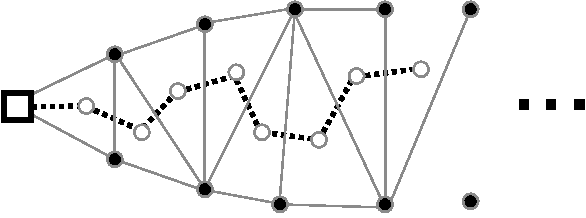
\includegraphics[scale=0.9]{figures/approach/trifail.pdf}}
		\caption[Limited ring size]{Limitations of triangulation and limited ring size.}
		\label{fig:trifail}
	\end{centering}
\end{figure}

A worst case scenario is depicted in Figure \ref{fig:trifail}. There can exist an arbitrary number if stations in the network but through the triangulation only one neighboring triangle to the transformer is built. After the first ring reaches its maximal number of stations there is no triangle for another ring left to start its construction. To counteract this bottleneck, the expansion rule described in \ref{backandforth} is relaxed for neighboring triangles of the transformer. This means that it is allowed to expand a triangle even though all three of its stations are already covered. In general this technique helps to find more solutions, although in the shown example it also would not work, since there only exist one available expansion option for each triangle. Another possible fix, is to increase the maximal number of allowed stations per ring. Similar to \ref{backandforth}, APMV just tries to restart the solution building process in the hope to find a different expansion order, which does not result in a restart. For the real network evaluated in this work, the number of restarts out of 1500 attempts in relation to the maximal ring size is depicted in Figure \ref{fig:restarts}. For a maximal ring size of 7 no solution could be found. Manual verification confirms that it is impossible to create a solution with only 7 stations per ring. In practice however manual verification is too time consuming, therefore sufficiently high iterations and ants per iteration have to be chosen. For 8 or more rings valid solutions are found by the algorithm. When the ring size is unlimited, almost all attempts lead to valid solutions. For critical ring sizes though runtime can be compromised considerably.
\begin{figure}[h]
	\begin{centering}
		{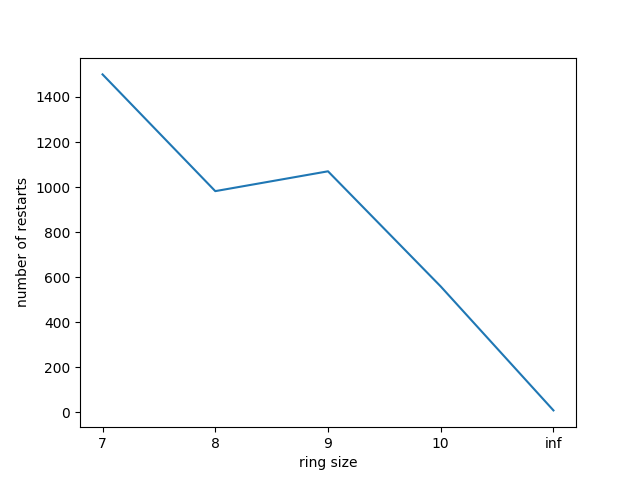
\includegraphics[scale=0.6]{figures/approach/restarts.png}}
		\caption[Number of restarts]{Number of restarts for different maximal ring sizes.}
		\label{fig:restarts}
	\end{centering}
\end{figure}


The approach of APMW is to prevent the expansion of critical triangles which could lead to faulty network structures already during the solution building process. The reason not to fix an invalid solution in a postprocessing step is that it seems more practical. Without preventing the expansion of certain triangles it is impossible to trace back and classify the exact reasons for a solution building attempt failed in hindsight. And without this classification of errors a reasonable "repairing" is very difficult. For future work it might be an interesting task to find a simple postprocessing procedure which fixes solutions created with an unrestricted expand method. This would prevent the need for restarting and could therefore speedup the algorithms runtime.

\subsection{Run Time}
%TODO: check Jonathan for runtime
